\documentclass{article}[18pt]
\usepackage{../../../../format}
\lhead{Networks and Systems - Networks}


\begin{document}
\begin{center}
\underline{\huge Data Link Layer}
\end{center}
\section{Frames}
\begin{itemize}
	\item Link layer accepts packets from the network layer, and encapsulates them into frames that it sends using the physical layer; reception is the opposite process
	\item The physical layer (below) is responsible for the transmission of raw sequences of bits
\end{itemize}
\begin{center}
	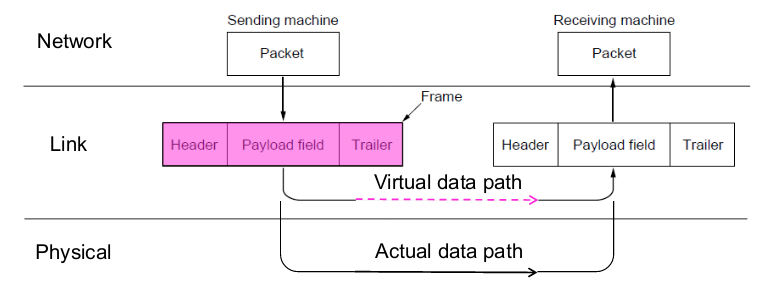
\includegraphics[scale=0.7]{frame}
\end{center}
\section{Framing methods}
\subsection{Byte count}
Frame begins with a count of the number of bytes in it - simple, but difficult to resynchronize after an error
\subsection{Headers and trailers}
We add a header (e.g. the length of the data, etc.) and a trailer (extra data that can be used e.g. error-detection or error-correction)
\begin{center}
	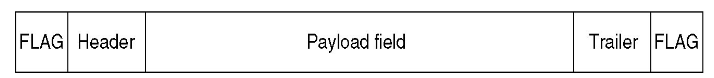
\includegraphics[scale=0.7]{flag}
\end{center}
Two adjacent frames are separated by a flag
\subsection{Byte stuffing}
Special flag bytes delimit frames; occurrences of flags in the data must (escapes) - longer, but easy to resynchronize after error
\begin{center}
	\includegraphics[scale=0.7]{"byte stuffing"}
\end{center}
\begin{center}
	\includegraphics[scale=0.7]{"byte stuffing1"}
\end{center}
\subsection{Bit stuffing}
\begin{center}
	\includegraphics[scale=0.7]{"bit stuffing"}
\end{center}
The flag is six consecutive ones. Within the data, a zero is stuffed after each five consecutive ones to void instances of the flag in the data\\
Bit stuffing
\begin{enumerate}[label=(\alph*)]
	\item The original data
	\item The data as they appear on the line
	\item The data as they are stored in receiver's memory after de-stuffing
\end{enumerate}
Sender:
\begin{itemize}
	\item Encloses packet (bit stream): 0 1 1 1 1 1 0
	\item Appends a 0 after each 1 1 1 1 1 in body (bit stuffing)
\end{itemize}
Receiver, upon receiving 0 1 1 1 1 1:
\begin{itemize}
	\item next bit 0: stuffed bit is removed
	\item next bit 1
	\begin{itemize}
		\item if next bit 0: end of frame marker
		\item if next bit 1: error
	\end{itemize}
\end{itemize}
\section{Error detection and correction}
\begin{itemize}
	\item Errors occur during frame transmission
	\item Two strategies to deal with error
	\begin{itemize}
		\item Include enough redundant information to help receivers deduce original data (error correcting)
		\item Include enough information to deduce an error occurred (error detecting)
		\item Neither error-correcting codes nor error-detecting codes can handle all possible errors
	\end{itemize}
\end{itemize}
EDC = Error detection and correction bit (redundancy)\\
D = Data protected by error checking, may include header fields\\
\\
Error detection is not 100\% reliable, protocol may miss some errors, but rarely
\begin{center}
	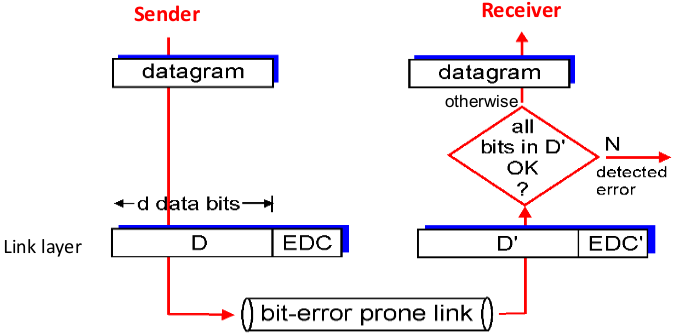
\includegraphics[scale=0.7]{EDC}
\end{center}
\section{Codeword}
\begin{itemize}
	\item A frame consists of m data (message) bits and r redundant (check) bits
	\item n-bit codewords with n=m+r
\end{itemize}
\section{Error codes}
Error codes add structured redundancy to data so errors can be either detected, or corrected
\subsection{Hamming codes}
\begin{defin}[Hamming distance]
The number of bit positions in which two codewords differ
\end{defin}
We will see a specific hamming code that corrects a single error:
\begin{itemize}
	\item Encoding: we number the data bits starting from one and skipping the powers of two. The powers of two are reserved for parity bits, the rest are message bits.
	\item Decoding: calculate all parities. If they are all OK, there was no error. If not, add up the positions of the incorrect ones - this gives us the position of the error
\end{itemize}
Hamming code gives a simple way to add check bits and correct up to a single bit error
\begin{itemize}
	\item Check bits are parity over subsets of the codeword
	\item Recomputing the parity sums (syndrome) gives the position of the error to flip, or 0 if there is no error
\end{itemize}
\section{Error detection}
\subsection{Parity}
Parity but is added as the modulo 2 sum of data bits\\
\\
\textbf{Single bit parity} - detect single bit errors\\
\\
\textbf{Two dimensional bit parity} - detect and correct single bit errors
\subsection{Checksum}
The sender:
\begin{enumerate}
	\item Data is divided into k segment each of m bits (normally 16 bit integers) and summed
	\item The 1s complement of the sum forms the checksum
	\item The checksum segment is sent along with the data segments
\end{enumerate}
The receiver
\begin{enumerate}
	\item All received segments are added
	\item The sum is complemented
	\item If the result is zero, the received data is OK; otherwise wrong
\end{enumerate}
\subsection{Cyclic Redundancy Check}
This is a more advanced technique, which uses manipulations with polynomials. This is one of the most commonly used error detection codes\\
\\
Basic approach:
\begin{itemize}
	\item Let M1 be the message of n-bits
	\item M1 is padded with CRC code and send it
	\item CRC is generated using a given polynomial P1 (or divisor)
	\item P1 is agreed between sender and receiver
	\item Receiver gets M1 + CRC and extracts the M1 using P1
\end{itemize}
\begin{center}
	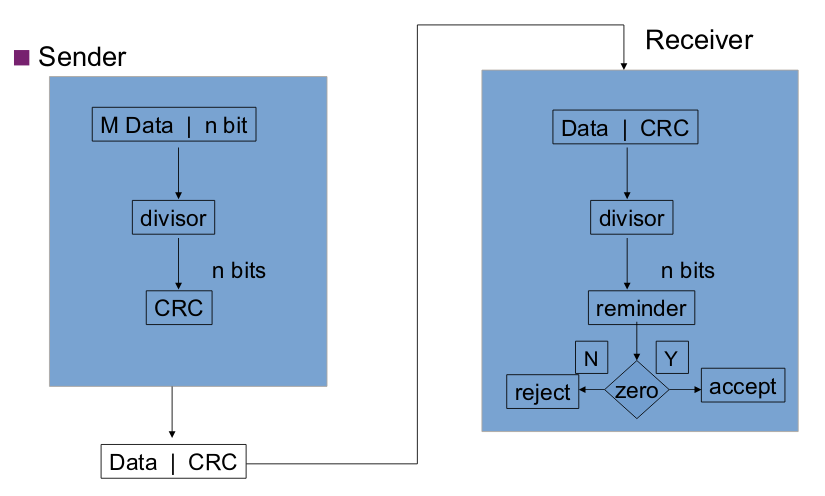
\includegraphics[scale=0.7]{CRC}
\end{center}

\end{document}